\documentclass{report}
\usepackage{longtable}
\usepackage{graphicx}
% When latex aborts with
%  pdfTeX error (ext4): \pdfendlink ended up in different nesting level than \pd
%  fstartlink.
% Comment that line with draft out and inpect the errornous page
\usepackage[pdfauthor={flonatel},%
%draft,%
pdftitle={Requirment for project},%
pdfsubject={Requirment description for project},%
pdfkeywords={placeholder for some keywords},%
pagebackref=true,%
pdftex, bookmarks=true, colorlinks=true]{hyperref}

\usepackage[a4paper]{geometry}

\usepackage[titles]{tocloft}
\usepackage{fancyhdr}

\setlength{\cftsubsecnumwidth}{4em}
\pagestyle{fancy}
\fancyhead{}
\fancyfoot{}
\fancyhead[L]{\rightmark}
\fancyfoot[R]{\thepage}
\fancyfoot[L]{Version \input{../artifacts/reqs-version.txt}}
\renewcommand{\headrulewidth}{0.4pt}
\renewcommand{\footrulewidth}{0.4pt}

\parindent0em

\begin{document}
\thispagestyle{empty}

\mbox{}

\vfill

{\LARGE\textbf{Requirements for project}}

\vfill

{\Large\textbf{written by You}}

\vfill

09. October 2010

\vfill

Requirements Version: \input{../artifacts/reqs-version.txt}

\vfill

\newpage

\tableofcontents

\newpage

\chapter{Status}
\section{Selected for Sprint}
\begin{longtable}{|r|c|p{7cm}||r|r|} \hline
\textbf{Prio} & \textbf{Chap} & \textbf{Requirement Id} & \textbf{EfE} & \textbf{Sum} \\ \hline\endhead
\end{longtable}\section{Assigned}
\begin{longtable}{|r|c|p{6.5cm}||r|l|l|} \hline
\textbf{Prio} & \textbf{Chap} & \textbf{Requirement Id} & \textbf{EfE} & \textbf{Person} & \textbf{Date} \\ \hline\endhead
\end{longtable}\section{Backlog}
\begin{longtable}{|r|c|p{7cm}||r|r|} \hline
\textbf{Prio} & \textbf{Chap} & \textbf{Requirement Id} & \textbf{EfE} & \textbf{Sum} \\ \hline\endhead
\end{longtable}\section{Requirements Elaboration List}
\begin{longtable}{|r|c|p{7cm}||r|r|} \hline
\textbf{Prio} & \textbf{Chap} & \textbf{Requirement Id} & \textbf{EfE} & \textbf{Sum} \\ \hline\endhead
10.00 & \ref{req1} & \nameref{req1} & 21 & 21 \\ \hline
10.00 & \ref{project} & \nameref{project} & 5 & 26 \\ \hline
\end{longtable}\section{Finished}
{\small \begin{longtable}{|c|p{5.5cm}||r|l|l|r|r|} \hline
\textbf{Chap} & \textbf{Requirement Id} & \textbf{EfE} & \textbf{Person} & \textbf{Date} & \textbf{Time} & \textbf{Rel} \\ \hline\endhead
\end{longtable}}\section{Statistics}
\begin{longtable}{rrl}
Start date & 2011-09-27 & \\ 
Not done & 0 & EfE units \\ 
Assigned & 0 & EfE units \\ 
Finished & 0 & EfE units \\ 
Finished (duration given) & 0 & EfE units \\ 
 & 0 & hours \\ 
\end{longtable}

% Output topic 'ReqsDocument'
\chapter{project}
This is placeholder for some introductional text.
% REQ 'project'
\section{project}\label{project}
\textbf{Description:} \textsl{project} \textbf{must} exists.

\textbf{Rationale:} The world needs a good, usable and free \textsl{project}.

\textbf{Solved by:} \ref{req1} \nameref{req1}

\par
{\small \begin{center}\begin{tabular}{rlrlrl}
\textbf{Id:} & project  & \textbf{Priority:} & 10.00  & \textbf{Owner:} & development\\ 
\textbf{Invented on:} & 2010-10-09  & \textbf{Invented by:} & flonatel  & \textbf{Status:} & not done \\ 
\textbf{Class:} & detailable  & & & \end{tabular}\end{center} }

% Output topic 'WhatsAbout'
\section{What's all about}
% REQ 'req1'
\subsection{req1}\label{req1}
\textbf{Description:} This \textbf{must} hold the description.

\textbf{Rationale:} This is a dependent requirement.

\textbf{Depends on:} \ref{project} \nameref{project}

\par
{\small \begin{center}\begin{tabular}{rlrlrl}
\textbf{Id:} & req1  & \textbf{Priority:} & 10.00  & \textbf{Owner:} & development\\ 
\textbf{Invented on:} & 2010-10-09  & \textbf{Invented by:} & flonatel  & \textbf{Status:} & not done \\ 
\textbf{Class:} & detailable  & & & \end{tabular}\end{center} }



\chapter{Statistics}
\section{Burndown diagram for Sprint}
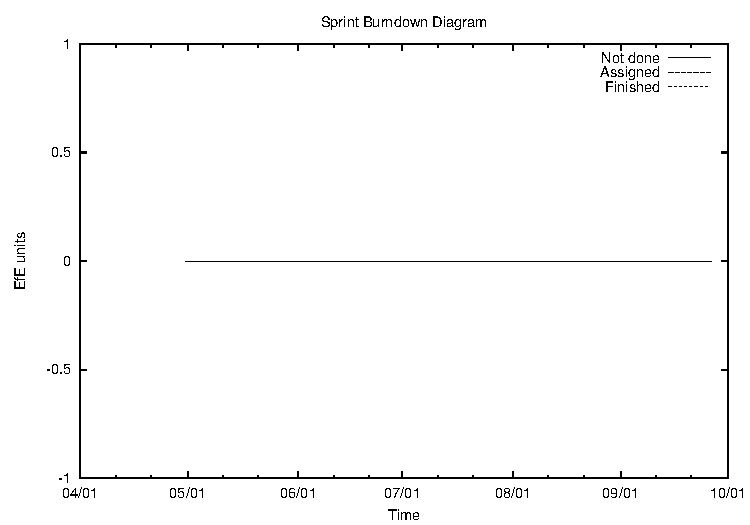
\includegraphics{../artifacts/stats_sprint_burndown.pdf}

\section{Burndown diagram for Project}
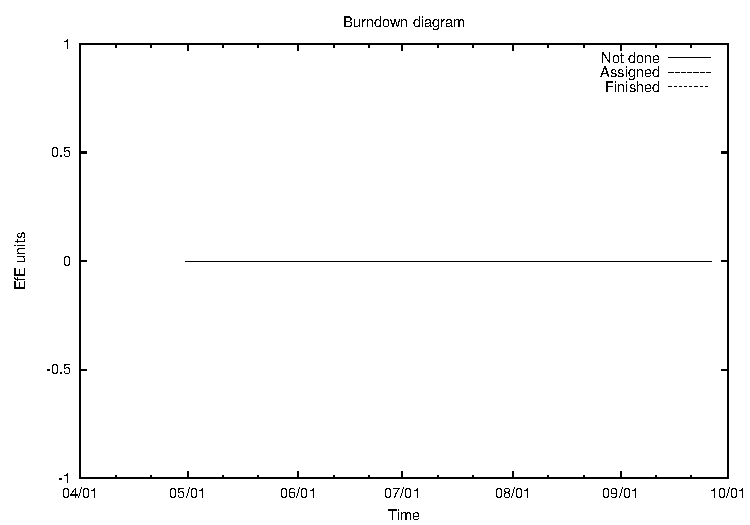
\includegraphics{../artifacts/stats_burndown.pdf}

\section{Requirements Count Statistics}
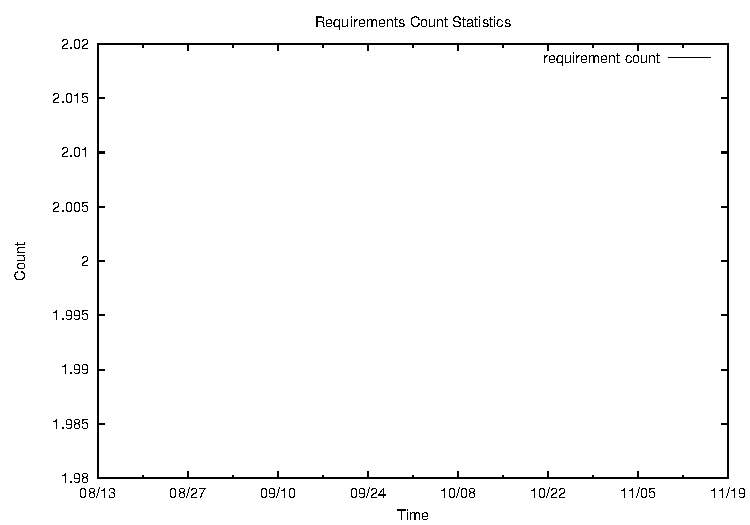
\includegraphics{../artifacts/stats_reqs_cnt.pdf}

\end{document}
